%%\begin{itemize}
%%\item {Experiments:} state of the art (open questions?) and estimates for low and high pt.
% \begin{itemize}
%\item {Observables:} RAA, v2, v3 for D, B mesons (when possible for both), event-shape engineering v2 analyses
%\item {Complementarity:} focus on complementarity (pt, y), provide plot of pt vs y for all experiments for a couple of observables.
%\end{itemize}
%%\item {Connection to theory:}  constrain c and b diffusion coefficients. Additional insights from v2(D) vs v2(pi) on event-by-event
%%\end{itemize}

%%\textbf{FIGURES}:
%%\begin{enumerate}
%%\item D RAA (ALICE+CMS)
%%\item B, non-prompt D, non prompt J/psi RAA (ALICE+CMS) 
%%\item D, B, non-prompt D, non prompt J/psi  v2 (ALICE+CMS)
%%\item summary figure to show complementarity: pt vs y for all experiments for a couple of observables
%%\item EsE D mesons (ALICE) + theory?
%%\item Theory: Ds ranges (Bayesian approach)
%%\item Theory: Ds ranges (using D and using D+B, Catania)
%%\end{enumerate}

\subsubsection{Nuclear modification factor and collective flow of heavy flavors}

One of the observables that can be used to study the medium effect on heavy-flavor meson production is nuclear modification factor ($R_{\mathrm{AA}}$), defined as the ratio of the PbPb yield to the pp cross-section scaled by the nuclear overlap function\cite{glauber}. In the view of the pQCD-based models, heavy quarks lose energy via radiative and collisional interactions with the medium constituents. The so-called ``dead-cone effect" is expected to reduce small-angle gluon radiation of heavy quarks when compared to both gluons and light quarks. At low $p_{\mathrm{T}}$, the production rate of heavy-flavor mesons in heavy-ion collisions is sensitive to the elastic energy loss of the heavy quark in medium, the nuclear shadowing effect in the initial state, and the recombination of the heavy quark with light quark at the hadronization stage. At high $p_{\mathrm{T}}$, the amplitude of nuclear modification factor is sensitive to the medium-induced radiative energy loss of heavy quark. Precise measurement of the $R_{\mathrm{AA}}$ could thus provide insights about the momentum dependence of the heavy quark energy loss, and provide important tests of QCD predictions in particular test the expected flavour dependence of the energy loss processes.

Another interesting observable is azimuthal anisotropy which can be characterized by the Fourier coefficients $v_{\mathrm{n}}$ in the azimuthal angle ($\phi$) distribution of the heavy-flavor hadron yield. A significant $v_{2}$ (eplliptic flow) is considered as evidence for the QGP formation. At low $p_{\mathrm{T}}$ the $v_{2}$ (elliptic flow) heavy-flavor hadron $v_{2}$ can help quantify the interaction strength of heavy quarks with the medium. $v_{2}$ can also be used to study the recombination process of heavy quarks with light quarks. At high $p_{\mathrm{T}}$, $v_{2}$ of heavy-flavor hadrons is sensitive to the path length dependence of heavy quark energy loss. Simultaneous prediction to $R_{\mathrm{AA}}$ and $v_{2}$ imposes a strict requirement to theoretical models.

\subsubsection{Experimental performance in CMS and ALICE}

Figure~\ref{fig:RAAv2.RAA} shows the projected performance of $R_{\mathrm{AA}}$ of multiple particles with $L_{\mathrm{int}}=10\;\mathrm{nb}^{-1}$. The left pad presents the projection of charged particles, $\mathrm{D}^{0}$, $\mathrm{B}^{+}$ and nonprompt (decayed from b-hadrons instead of being fragmented from charm) $J/\psi$ which can be measured by CMS. The middle pad shows the projection of $\mathrm{D}^{0}$ and nonprompt $J/\psi$, and the right pad shows $\mathrm{B}^{+}$ ($\rightarrow \mathrm{D}^{0}\pi^{+}$) estimated from ALICE. The center values of $R_{\mathrm{AA}}$ are taken from \cite{raatheory}. With the high luminosity and the Inner Tracker System Upgrade in ALICE, the $R_{\mathrm{AA}}$ of light hadrons, c-hadrons and b-hadrons can be clearly separated in a wide kinematic range. Also, the precise measurement could provide a strong constraint on theoretical models.

\begin{figure}[ht]
  \begin{center}
    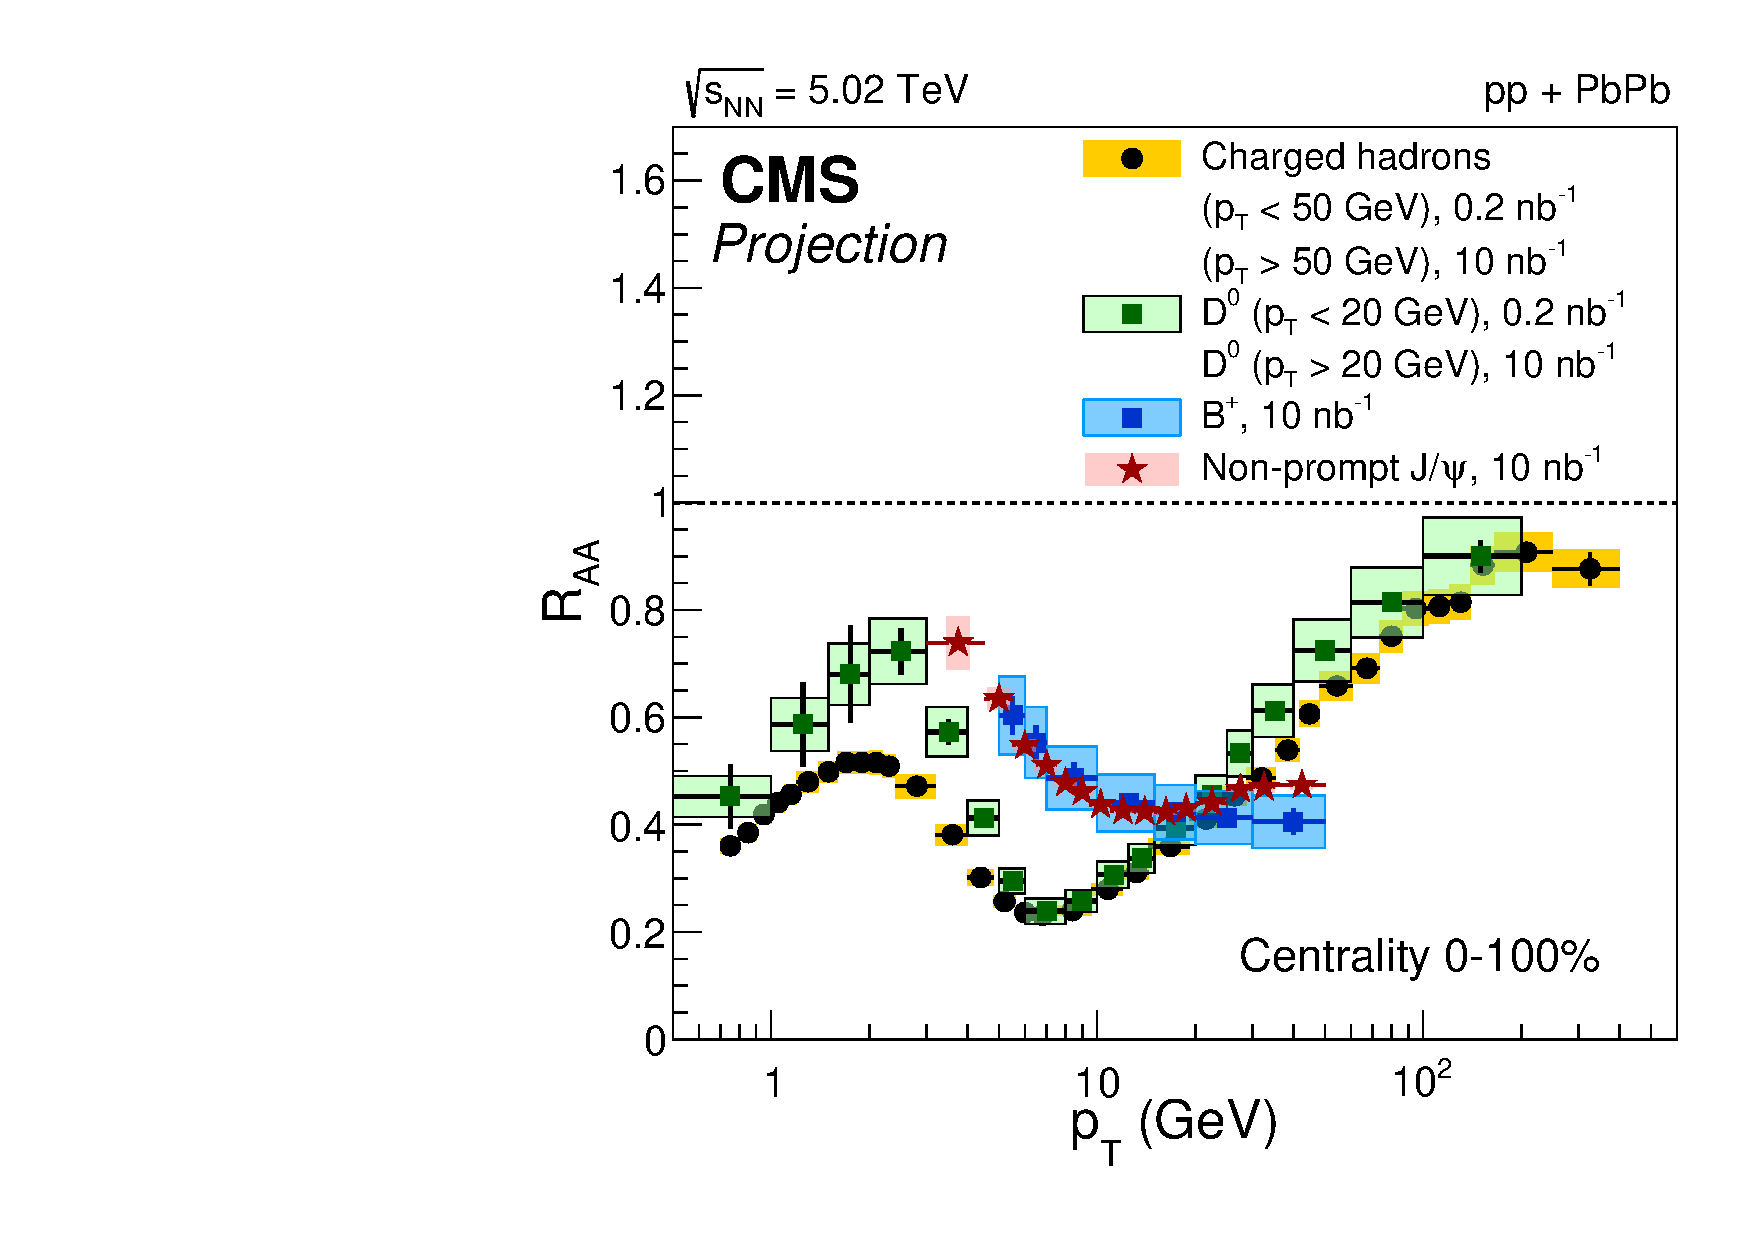
\includegraphics[width=0.32\textwidth]{hf/figures/cRAA_lumiTG_10_lumiMB_0_v2_right.pdf}
    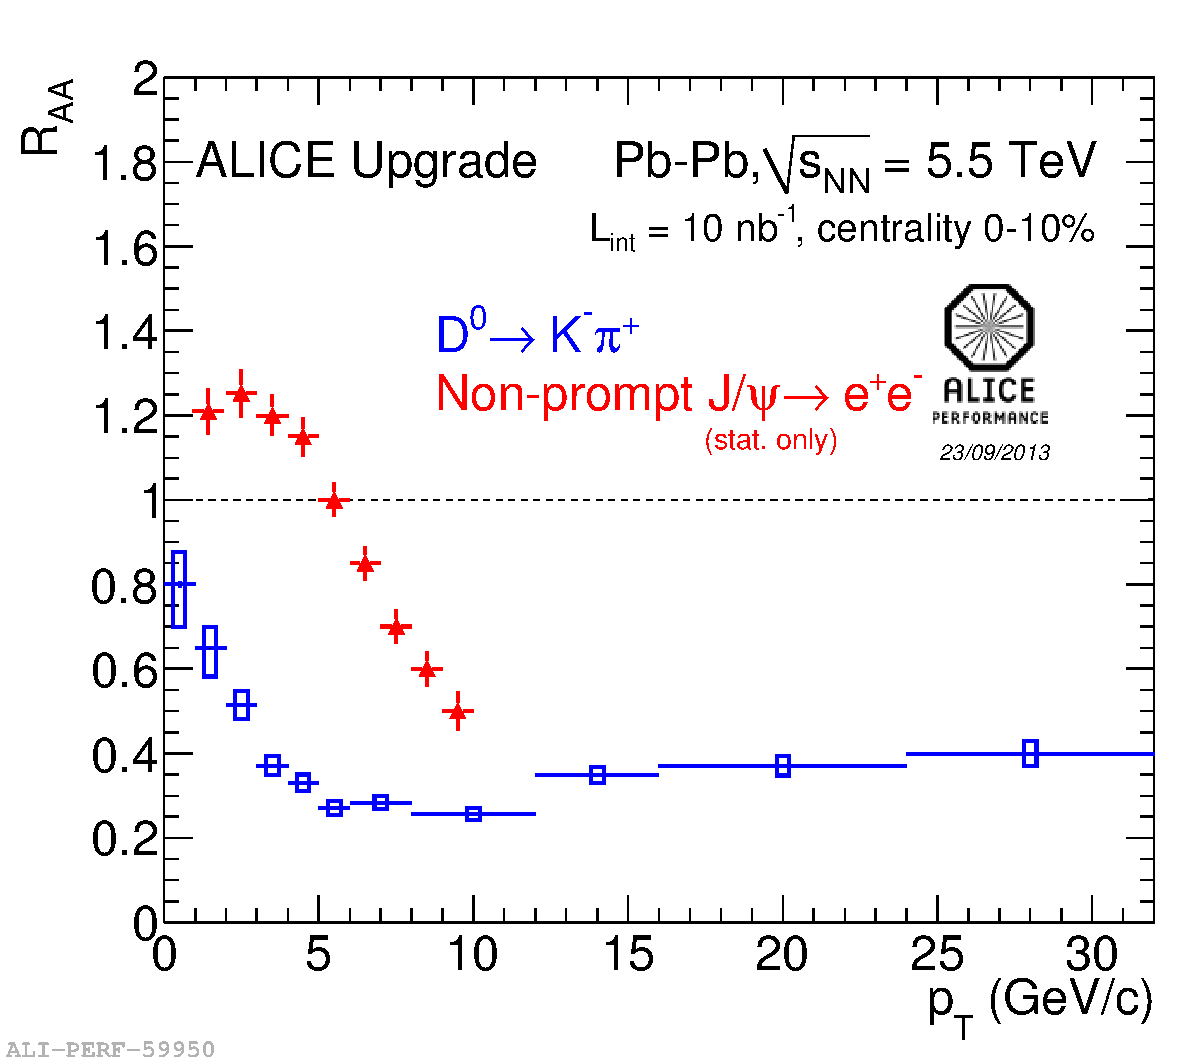
\includegraphics[width=0.32\textwidth]{hf/figures/2013-Oct-24-D0BJpsiRAAprompt_TDR_logo.pdf}
    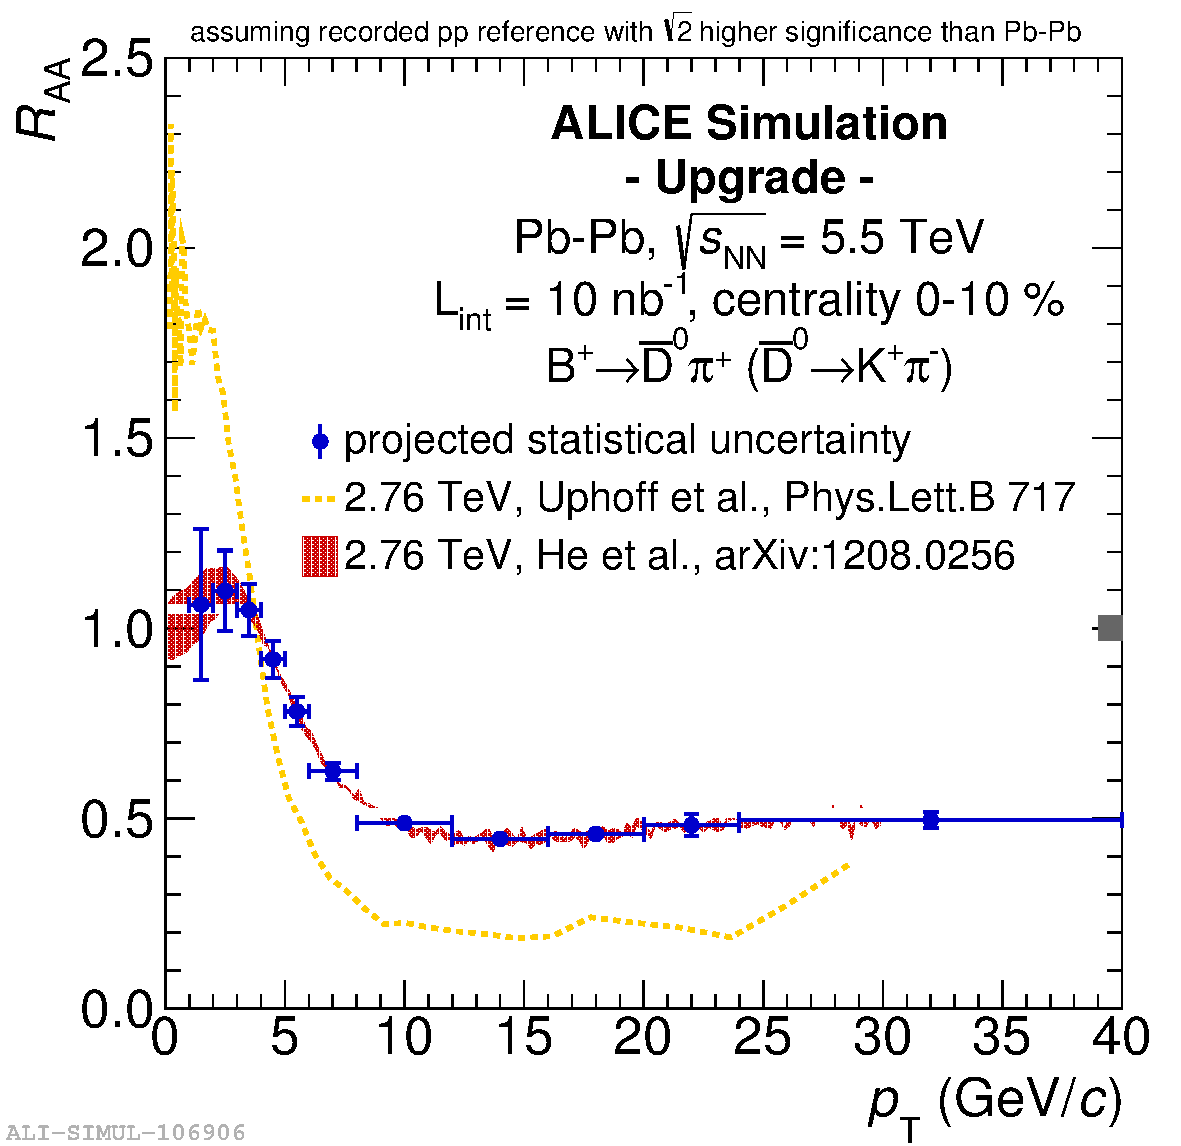
\includegraphics[width=0.32\textwidth]{hf/figures/2016-Jun-10-BMeson_wPID_Raa.pdf}
    \caption{Nuclear modification factors of charged particles, $\mathrm{D}^{0}$, $\mathrm{B}^{+}$ and nonprompt $J/\psi$ from CMS (left), $\mathrm{D}^{0}$, nonprompt $J/\psi$ (middle) and nonprompt $\mathrm{D}^{0}$ (right) from ALICE with the PbPb statistics expected with $10$ $\mathrm{nb}^{-1}$.}
    \label{fig:RAAv2.RAA}
  \end{center}
\end{figure}


Figure~\ref{fig:RAAv2.v2charm} shows the projected performance of $v_{2}$ of charm hadrons with $L_{\mathrm{int}}=10\;\mathrm{nb}^{-1}$. The left pad shows the projection of $\mathrm{D}^{0}$ from CMS, and the charged particle $v_{2}$ is overlaped for comparison. The right pad presents the projection of $\mathrm{D}^{0}$, $\mathrm{D}_{s}^{+}$ and $\lambda_{c}^{+}$ which could be measured by ALICE. The center values are taken from \cite{v2charmtheory}. Precise measurement of charm hadron $v_{2}$ could help study the thermalization of heavy quarks and the wide kinematic range allows to get insights on different process as coalescence hadronization and energy loss. Figure~\ref{fig:RAAv2.v2beauty} shows the projeted performance of $v_{2}$ of beauty hadrons which ALICE could measure with $L_{\mathrm{int}}=10\;\mathrm{nb}^{-1}$. The left pad presents the projection of nonprompt $\mathrm{D}^{0}$ and nonprompt $J/\psi$ while the right pad shows the projection of $\mathrm{B}^{+}$. This will possible become the first precise measurement on the flow of b quarks.

\begin{figure}[ht]
  \begin{center}
    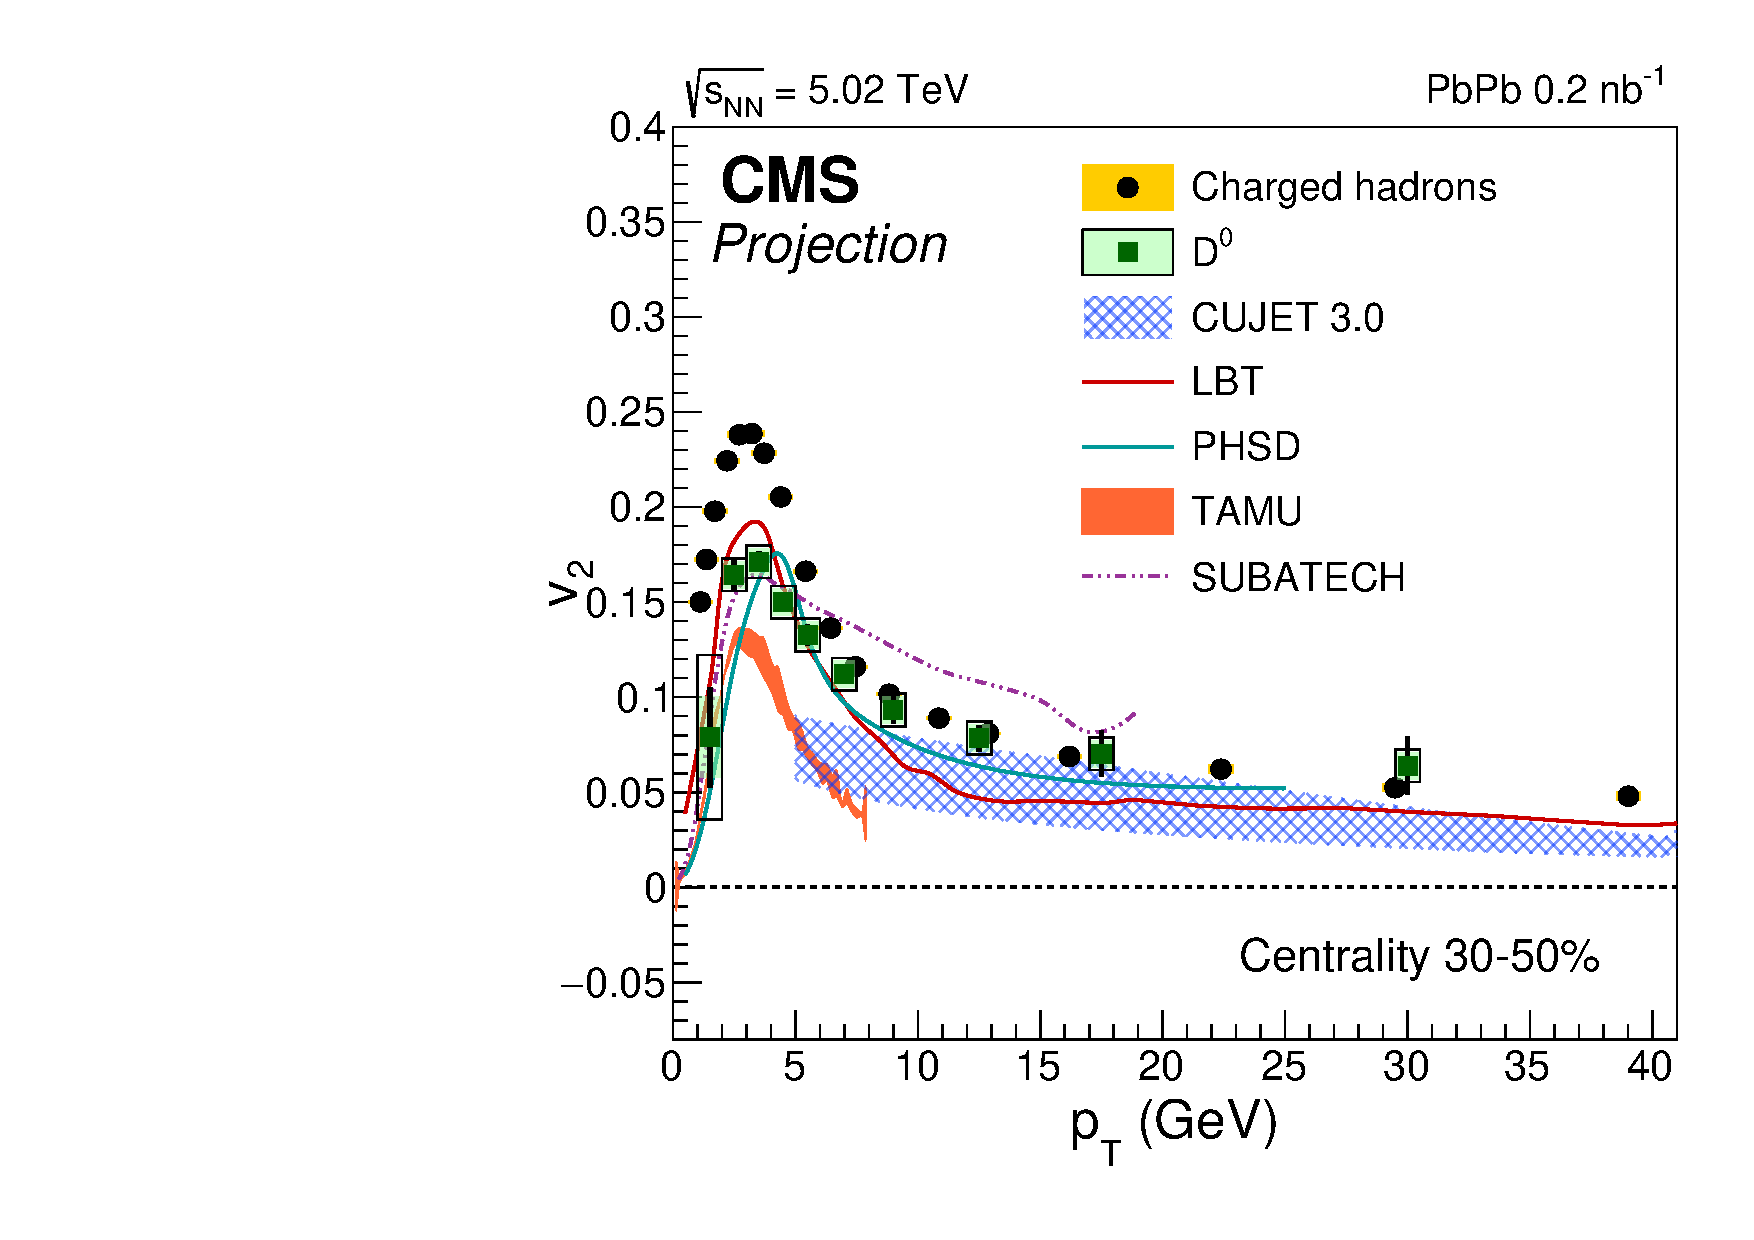
\includegraphics[width=0.49\textwidth]{hf/figures/cV2_lumiMB_0_wTheory_right.pdf}
    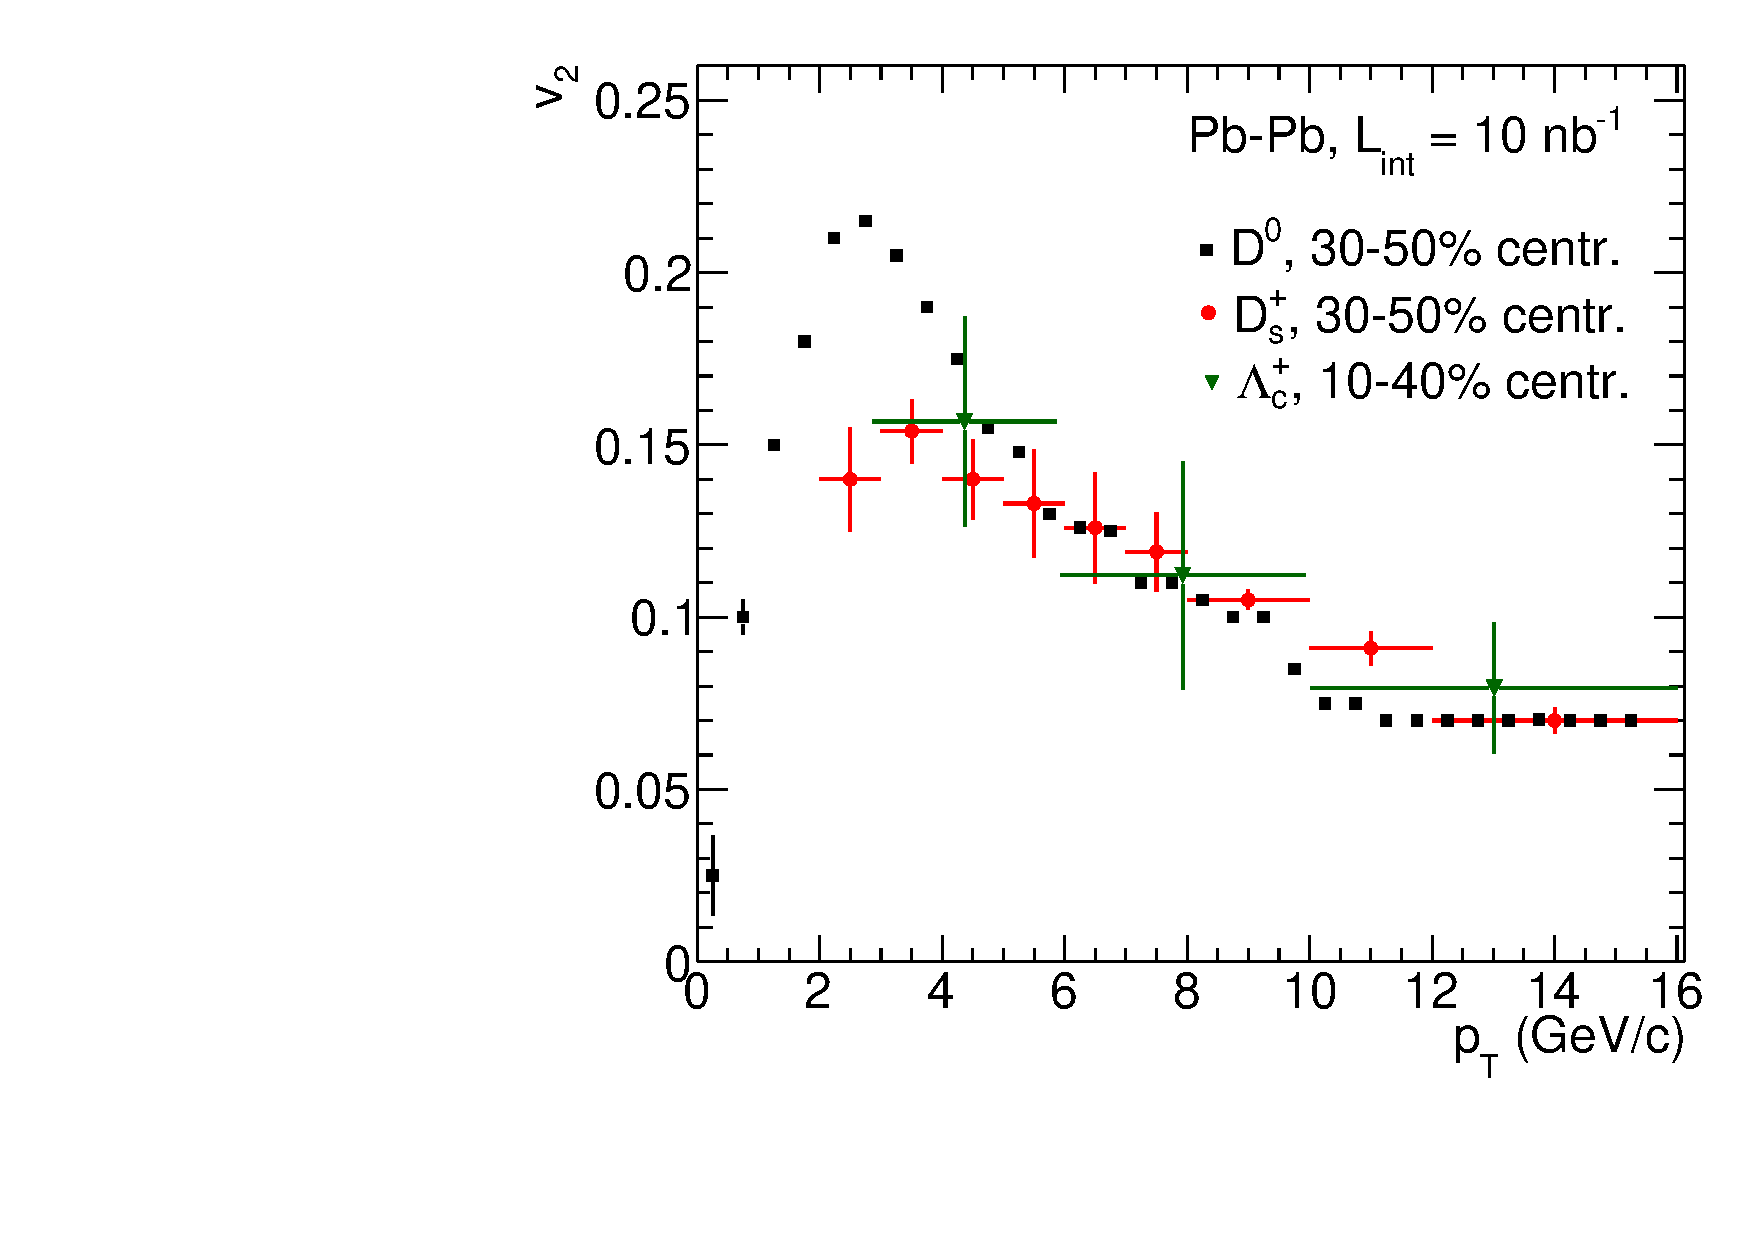
\includegraphics[width=0.49\textwidth]{hf/figures/D0DsLc_v2_TDR.pdf}
    \caption{$v_{2}$ of charged particles and $\mathrm{D}^{0}$ from CMS (left), charm hadrons ($\mathrm{D}^{0}$, $\mathrm{D}_{s}^{+}$, $\lambda_{c}^{+}$) from ALICE (right) with the PbPb statistics expected with $10$ $\mathrm{nb}^{-1}$.}
    \label{fig:RAAv2.v2charm}
  \end{center}
\end{figure}
\begin{figure}[ht]
  \begin{center}
    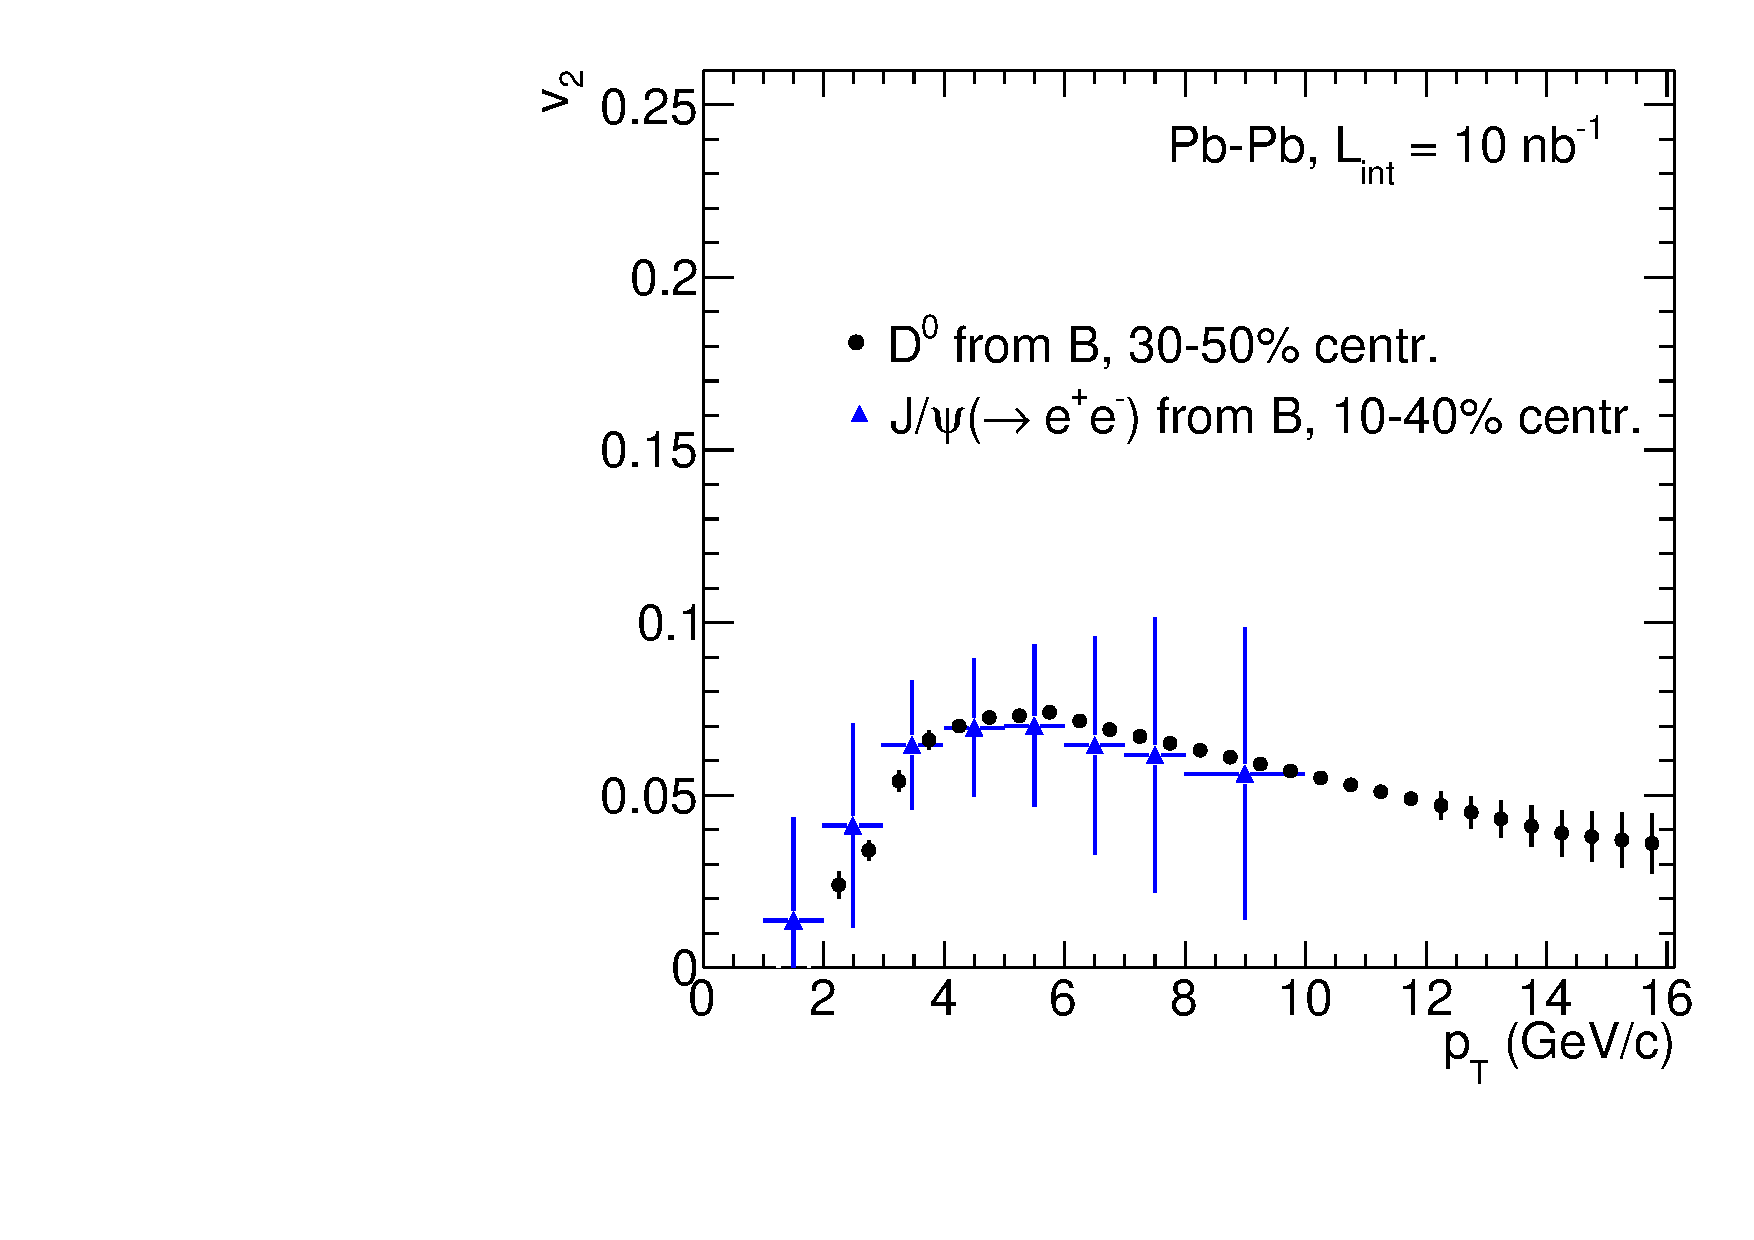
\includegraphics[width=0.49\textwidth]{hf/figures/D0fromB_JpsifromB_v2_TDR.pdf}
    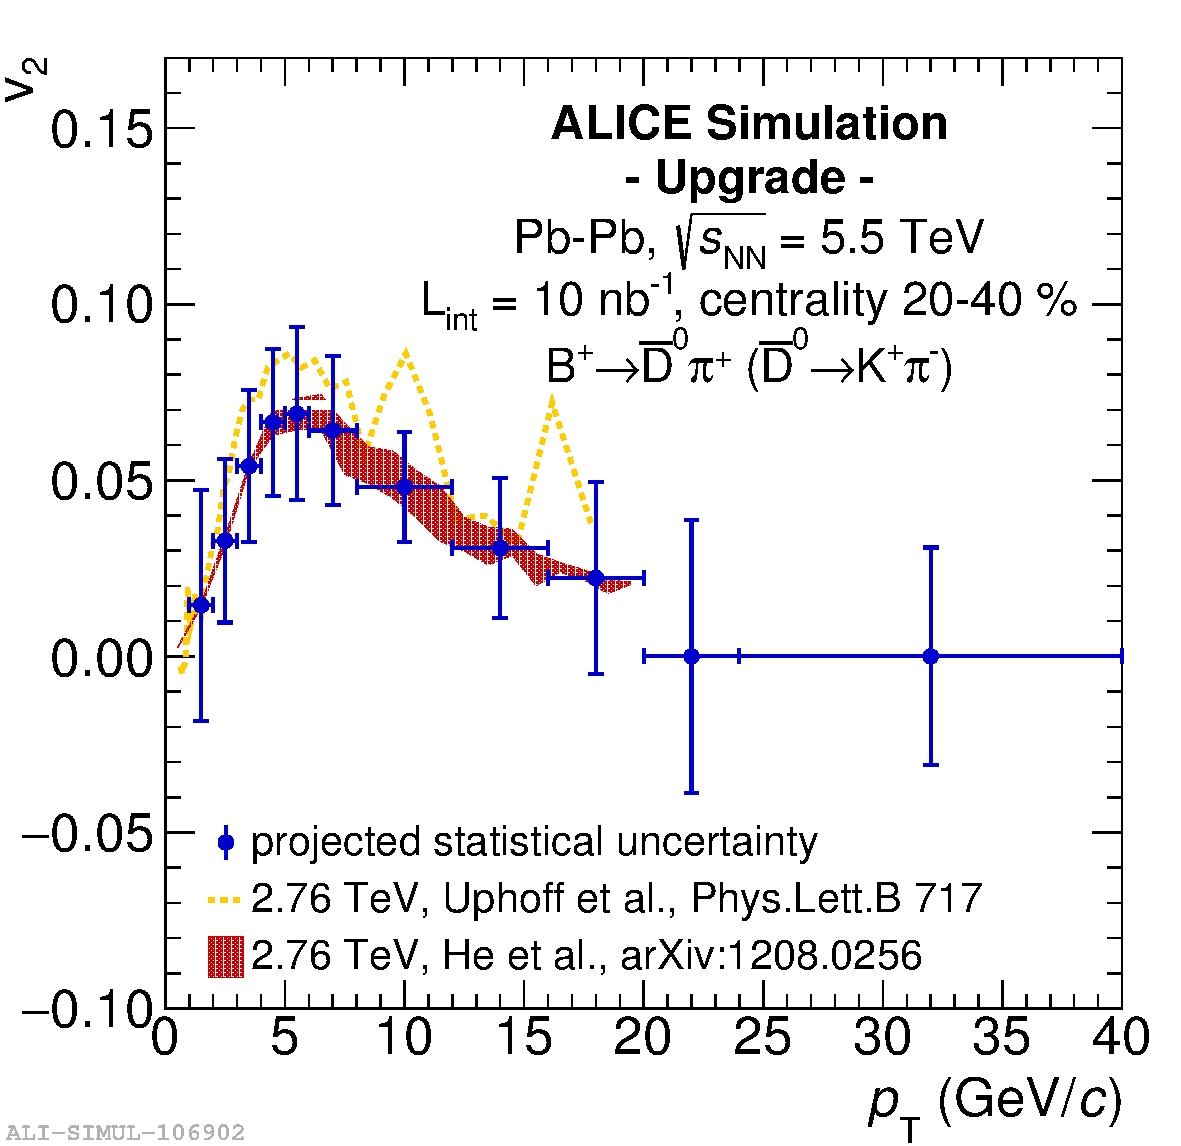
\includegraphics[width=0.49\textwidth]{hf/figures/2016-Jun-10-PlotAllResults_v2FinalEstimate_20-40.pdf}
    \caption{$v_{2}$ of nonprompt $\mathrm{D}^{0}$ and nonprompt $J/\psi$ (left), $\mathrm{B}^{+}$ ($\rightarrow \mathrm{D}^{0}$) (right) from ALICE with the PbPb statistics expected with $10$ $\mathrm{nb}^{-1}$.}
    \label{fig:RAAv2.v2beauty}
  \end{center}
\end{figure}

\subsubsection{Constraining heavy quark transport coefficient}
Over the past few years, many theoretical efforts have been taken to understand the transport properties of heavy flavors in the medium. Although the mechanisms can widely vary among different theoretical models, transport coefficients can be used to compare these models. Despite successful estimation of some transport properties like the shear viscosity, the most basic energy loss mechanism are not yet understood and the diffusion coefficient ($D_{s}$) is to be determined. So far simultaneously describing $R_{\mathrm{AA}}$ and $v_{\mathrm{n}}$ is still top challenge for many models, the future precise data will be able to constrain the heavy quark diffusion coefficient in QGP, potentially distinguish different models and greatly improve our understanding to the interaction mechanism between heavy quarks and the medium.

\begin{figure}[ht]
  \begin{center}
    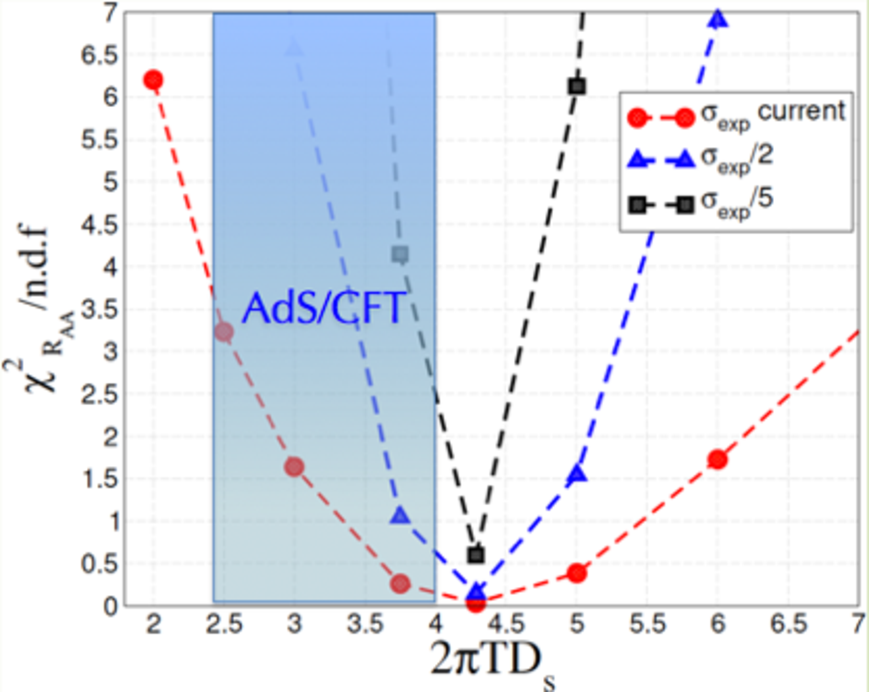
\includegraphics[width=0.49\textwidth]{hf/figures/Greco.pdf}
    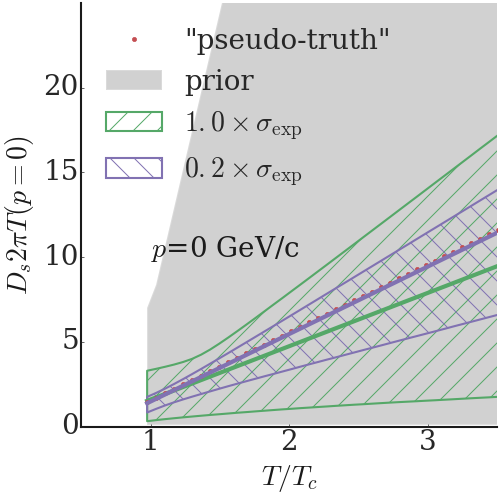
\includegraphics[width=0.49\textwidth]{hf/figures/Plot_D2piT_posterior_p0.png}
    \caption{Normalized $\chi^{2}$ as a function of spatial diffusion coefficient ($2\pi TD_{s}$) under different experimental precision from AdS/CFT (left). Coefficient range in the phase plane of $2\pi TD_{s}$ vs. $T_{c}$ under different experimental precision with LBT model (right).}
    \label{fig:RAAv2.Dstheory}
  \end{center}
\end{figure}

Figure~\ref{fig:RAAv2.Dstheory} shows the constrain power of experimental result of $R_{\mathrm{AA}}$ and $v_{\mathrm{n}}$ on the diffusion coefficient under different experimental precision. The left pad is Normalized $\chi^{2}$ as a function of spatial diffusion coefficient ($2\pi TD_{s}$) from AdS/CFT. The right pad shows the coefficient range in the phase plane of $2\pi TD_{s}$ vs. $T_{c}$ with LBT model.

\subsubsection{Event Shape Engineering}
\textbf{to add}
